\chapter{Figuren UML}
\label{appendix:FiguresUML}

\begin{graphic}
    \captionsetup{type=figure}
    \caption{Klassendiagram ItemValue}
    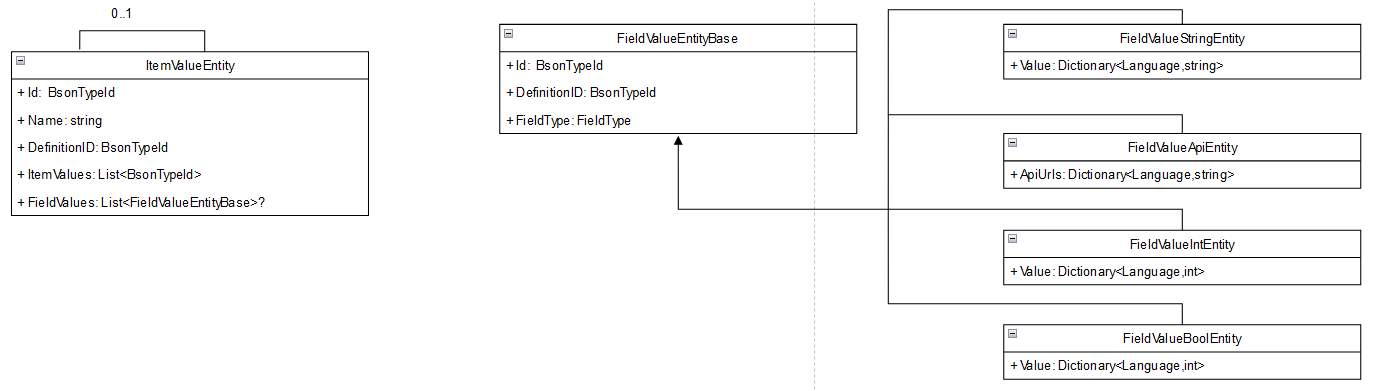
\includegraphics[scale=0.4,angle=90]{ItemValueEntityClassDiagram.png}
    \label{appendix:ItemValueEntityClassDiagram}
\end{graphic}

\begin{graphic}
    \captionsetup{type=figure}
    \caption{Klassendiagram  ItemDefinition}
    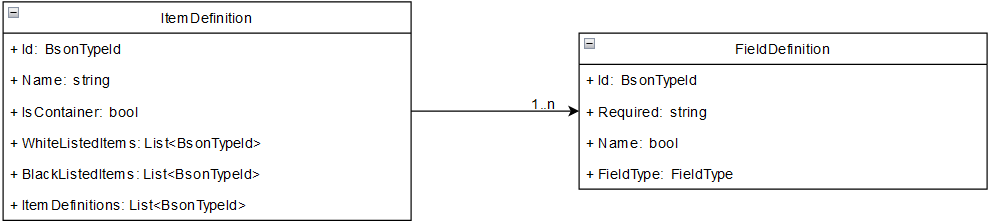
\includegraphics[scale=0.8,angle=90]{ItemDefinitionClassDiagram.png}
    \label{appendix:ItemDefinitionClassDiagram}
\end{graphic}

\whitespace[2]
\begin{graphic}
    \captionsetup{type=figure}
    \caption{Klassendiagram VisualComponent}
    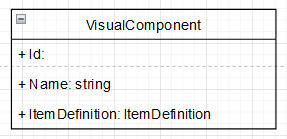
\includegraphics[scale=0.8]{VisualComponentEntityClassDiagram.png}
    \label{appendix:VisualComponentEntityClassDiagram}
\end{graphic}

\whitespace[2]
\begin{graphic}
	\captionsetup{type=figure}
	\caption{Klassendiagram ItemVisual}
	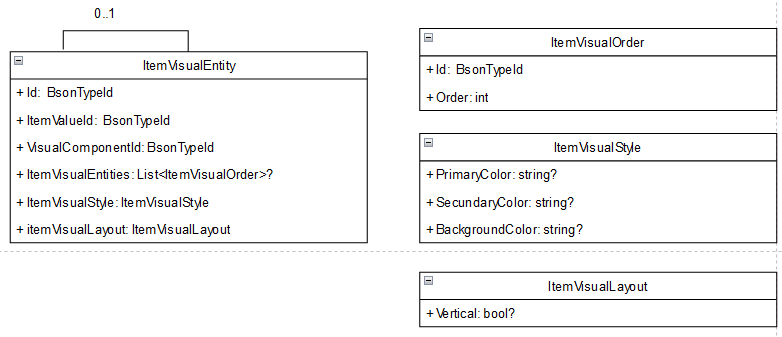
\includegraphics[scale=0.8,angle=90]{ItemVisualEntityClassDiagram.png}
	\label{appendix:ItemVisualEntityClassDiagram}
\end{graphic}

\whitespace[2]
\begin{graphic}
	\captionsetup{type=figure}
	\caption{Klassendiagram ItemVisualDTO}
	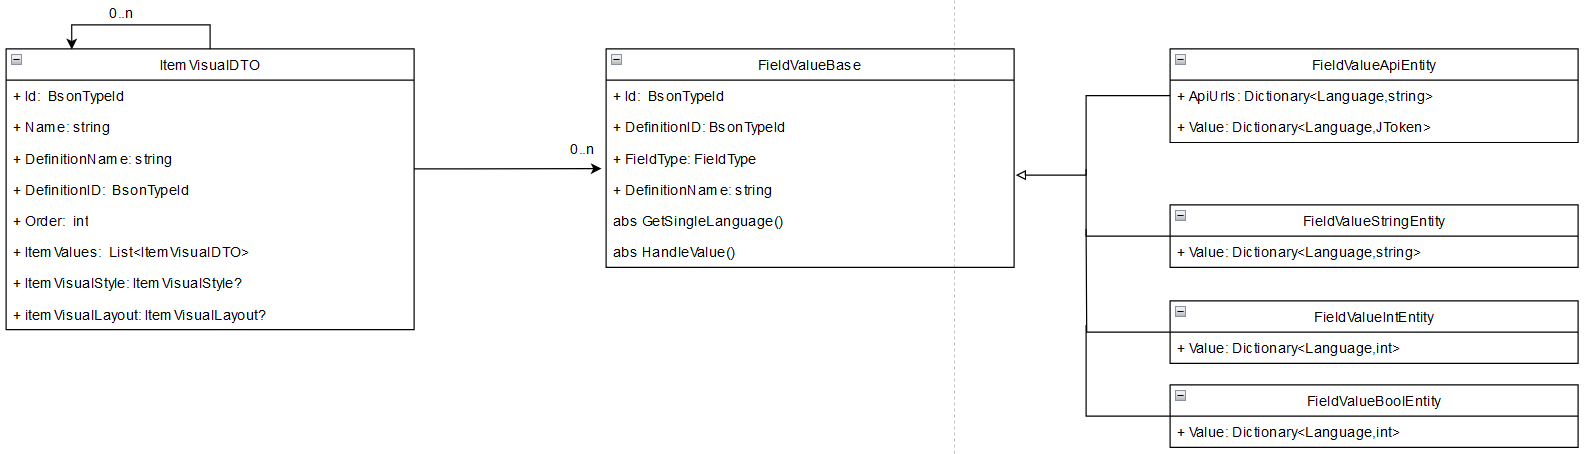
\includegraphics[scale=0.55,angle=90]{ItemVisualDTO.png}
	\label{appendix:ItemVisualDTOClassDiagram}
\end{graphic}

\begin{graphic}
    \captionsetup{type=figure}
    \caption{Klassendiagram ItemValue}
    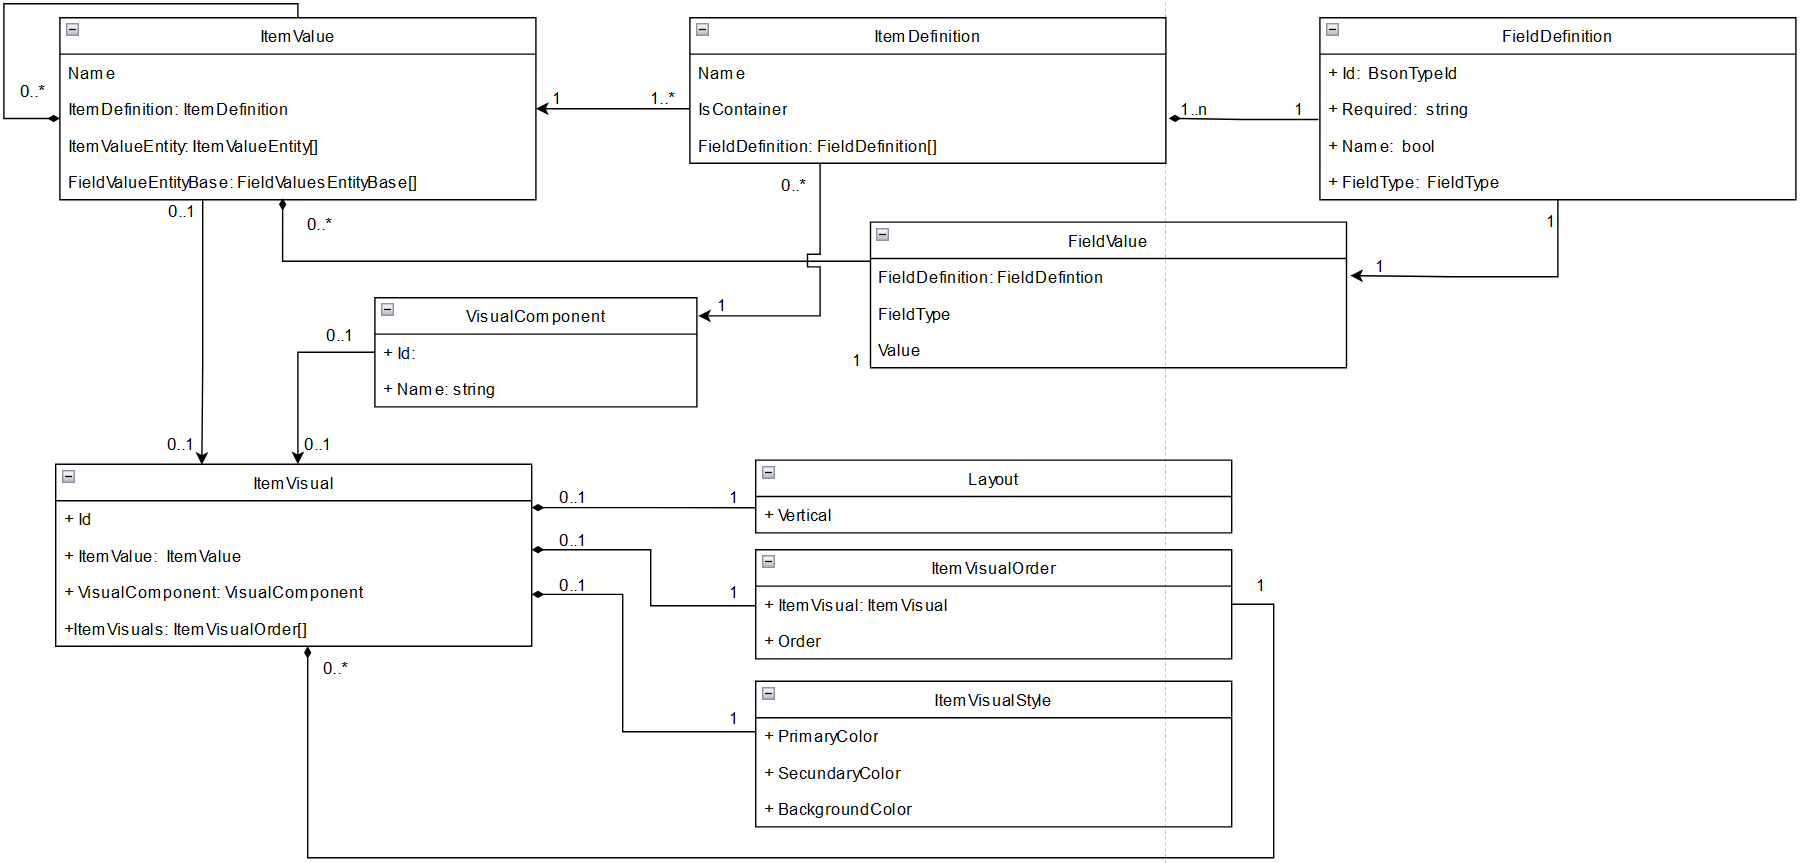
\includegraphics[scale=0.5,angle=90]{ClassDiagramEntireSystem.png}
    \label{appendix:ClassDiagramEntireSystem}
\end{graphic}
